\documentclass[newPxFont]{beamer}
%\documentclass[handout]{beamer} % Раздаточный материал (на слайдах всё сразу)
%\documentclass[aspectratio=169]{beamer} % Соотношение сторон


\usetheme{LTX}

%-=-=-=-=-=-=-=-=-=-=-=-=-=-=-=-=-=-=-=-=-=-=-=-=
%        LOADING PACKAGES
%-=-=-=-=-=-=-=-=-=-=-=-=-=-=-=-=-=-=-=-=-=-=-=-=
\usepackage{amsmath,amsfonts,amssymb,amsthm,mathtools}  % Тут мы подключаем пакеты для математики!

%%%%%%%%%%%%%%%%%%%%%%%% Шрифты %%%%%%%%%%%%%%%%%%%%%%%%%%%%%%%%%

\usepackage{fontspec}         % пакет для подгрузки шрифтов
\setmainfont{HelveticaNeueCyr}   % задаёт основной шрифт документа

% why do we need \newfontfamily:
% http://tex.stackexchange.com/questions/91507/
\newfontfamily{\cyrillicfonttt}{HelveticaNeueCyr}
\newfontfamily{\cyrillicfont}{HelveticaNeueCyr}
\newfontfamily{\cyrillicfontsf}{HelveticaNeueCyr}
% Иногда тех не видит структуры шрифтов. Эти трое бравых парней спасают ситуацию и доопределяют те куски, которые Тех не увидел.

\usepackage{unicode-math}     % пакет для установки математического шрифта
\setmathfont{Asana Math}      % шрифт для математики

\usepackage{polyglossia}      % Пакет, который позволяет подгружать русские буквы
\setdefaultlanguage{russian}  % Основной язык документа
\setotherlanguage{english}    % Второстепенный язык документа

%%% Работа с картинками
\usepackage{graphicx}  % Для вставки рисунков
\graphicspath{{images/}{images2/}}  % папки с картинками
\setlength\fboxsep{3pt} % Отступ рамки \fbox{} от рисунка
\setlength\fboxrule{1pt} % Толщина линий рамки \fbox{}
\usepackage{wrapfig} % Обтекание рисунков текстом

%%% Работа с таблицами
\usepackage{array,tabularx,tabulary,booktabs} % Дополнительная работа с таблицами
\usepackage{longtable}  % Длинные таблицы
\usepackage{multirow} % Слияние строк в таблице

%%% Программирование
\usepackage{etoolbox} % логические операторы

%%% Другие пакеты
\usepackage{multicol} % Несколько колонок

%%% Картинки
\usepackage{tikz} % Работа с графикой
\usepackage{pgfplots}
\usepackage{pgfplotstable}


\usepackage{xcolor}
\usepackage{hyperref}
\hypersetup{				
    unicode=true,           % позволяет использовать юникодные символы
    colorlinks=true,       	% true - цветные ссылки, false - ссылки в рамках
    urlcolor=blue,          % цвет ссылки на url
    linkcolor=red,          % внутренние ссылки
	hyperindex=true         % сделать ли ссылку кликабельной?
	breaklinks=true         % если ссылка не умещается в одну строку, разбивать    
	                        % ли ее на две части?
}
\usepackage{verbatim}
\usepackage{fancyvrb}
\usepackage{mdframed}

\usepackage{chronology}

\renewcommand{\event}[3][e]{%
  \pgfmathsetlength\xstop{(#2-\theyearstart)*\unit}%
  \ifx #1e%
    \draw[fill=black,draw=none,opacity=0.5]%
      (\xstop, 0) circle (.2\unit)%
      node[opacity=1,rotate=45,right=.2\unit] {#3};%
  \else%
    \pgfmathsetlength\xstart{(#1-\theyearstart)*\unit}%
    \draw[fill=black,draw=none,opacity=0.5,rounded corners=.1\unit]%
      (\xstart,-.1\unit) rectangle%
      node[opacity=1,rotate=45,right=.2\unit] {#3} (\xstop,.1\unit);%
  \fi}%

\title{Уютный факультатив по \LaTeX}
\subtitle{Шрифты, картинки и таблицы}
\date{\today}

\begin{document}

\begingroup
\setbeamercolor{background canvas}{bg = LTXDarkGrey}
\begin{frame}[plain]
\centering  
\includegraphics[width=0.7\linewidth]{font.jpg}	
\end{frame}
\endgroup 

\maketitle
 
\section{Шрифты}  
 
\begin{frame}{Кодировка} 
Кодировка - способ представления в памяти компьютера цифр, букв и всех остальных знаков. 

\centering 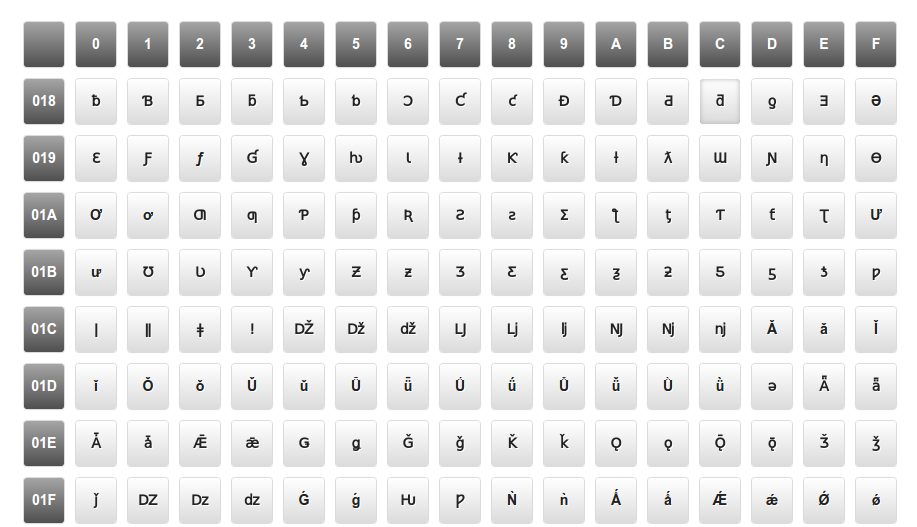
\includegraphics[width=0.7\linewidth]{codirovka.png}	
\end{frame}

\begin{frame}{Откуда берутся кракозябры} 
\centering 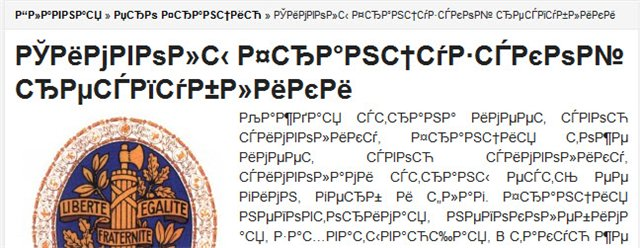
\includegraphics[width=0.7\linewidth]{krakozabr.jpg}	
\vspace{0.3cm}

\begin{itemize}
\item Мало памяти, 7 бит достаточно для всего (256 ячеек)
\item 127 ячеек - основа: символы, цифры, латиница
\item 128 ячеек - другое: кириллица, немецкий и т.п.
\item Каждое новое заполнение 128 символов $\Rightarrow$ новая кодировка
\end{itemize}
\end{frame}


% когда-то памяти было совсем немного и всем компьютерам было достаточно 7 бит для представления всех нужных символов (цифры, строчный\прописной латинский алфавит, куча знаков и так называемые управляемые символы — все возможные 127 номеров были кому-то отданы). Кодировка в это время была одна — ASCII. Шло время, все были счастливы, а кто не был счастлив (читай — кому не хватало знака "©" или родной буквы «щ») — использовали оставшиеся 128 знаков на свое усмотрение, то есть создавали новые кодировки. Так появились и ISO-8859-1, и наши (то есть кириличные) cp1251 и KOI8. Вместе с ними появилась и проблема интерпретации байтов типа 0b1******* (то есть символов\чисел от 128 и до 255) — например, 0b11011111 в кодировке cp1251 это наша родная «Я», в тоже время в кодировке ISO-8859-1 это греческая немецкая Eszett (подсказывает Moonrise) "ß". Ожидаемо, сетевая коммуникация и просто обмен файлами между разными компьютерами превратились в чёрт-знает-что.


\begin{frame}{Юникод} 
\begin{itemize}
\item Собрались великие умы в 1991 году и юникод придумали!
\end{itemize}

\centering  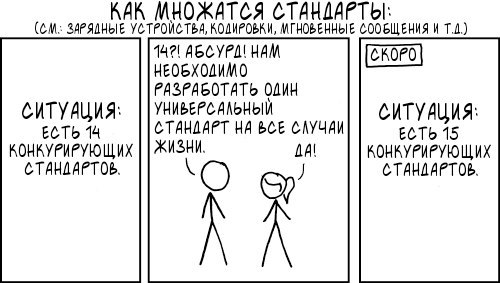
\includegraphics[width=0.7\linewidth]{stdcom.jpg}	
\end{frame}


\begin{frame}{Старый путь и новый путь}

\begin{block}{Движок pdf-LaTeX}
\verb|\usepackage[british,russian]{babel}| \% выбор языка для документа
\verb|\usepackage[utf8]{inputenc}|         \% задание utf8 кодировки исходного tex файла
\verb|\usepackage[X2,T2A]{fontenc}|        \% кодировка
\end{block}

\begin{block}{Движок XeLaTeX}
\verb|\usepackage{fontspec}|            \% пакет для подгрузки шрифтов
\verb|\setmainfont{HelveticaNeueCyr}|   \% задаёт основной шрифт документа

\verb|\usepackage{unicode-math}|     \% пакет для установки математического шрифта
\verb|\setmathfont{Asana Math}|      \% шрифт для математики

\verb|\usepackage{polyglossia}|      \% Пакет, который позволяет подгружать русские буквы
\verb|\setdefaultlanguage{russian}|  \% Основной язык документа
\verb|\setotherlanguage{english}|    \% Второстепенный язык документа
\end{block}
\end{frame}

\begin{frame}{Мольба к аудитории} 
Если в вас есть хоть что-то святое, используйте всегда utf-8, 
\end{frame}

\section{Картинки} 

\begin{frame}{Векторные и растровые картинки} 
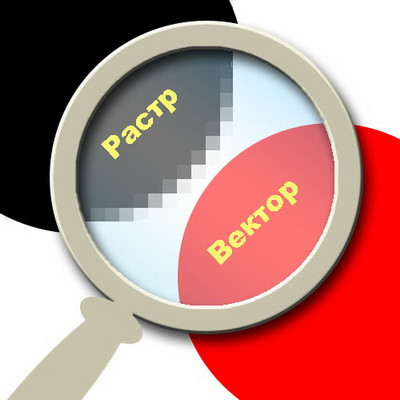
\includegraphics[scale=0.8]{rv.jpg}
\end{frame}

\begin{frame}{ } 

\end{frame}

\section{Таблицы} 

% Показать нечитаемую таблицу и буктабс!
\begin{frame}{ } 

\end{frame}

\begin{frame}{ } 

\end{frame}

\end{document}

